\documentclass{article}
\usepackage{graphicx,amsmath}
\begin{document}
\title{Discontinuities in Finf in some modes are not due to discontinuities in nmax index}
\author{Steven Dorsher}
\maketitle

I investigated the discontinuities in Finf as well as discontinuities in the order selected by bestfinfscript as the best choice order to begin the extrapolation for Finf. This is based on the maximum order at which this extrapolation is defined. The curve of Finf values as a function of starting DG order for the extrapolation approaches a constant for all modes I have checked, in a manner that appears like a shallow exponential. This motivates the choice of maximum possible starting order for the ``best'' choice finf value. Above some maximum starting order, finf is undefined due to a bad g(alpha) ratio (less than 0.5). This is due to round off noise causing the curve to fail to behave exponentially, and is worse with higher orders, but appears to be a function of the time as well in a somewhat random manner (round off noise explains the randomness).

For the ``best'' finf versus time, there are discontinuitites in a few specific modes, as seen yesterday. First I plotted time versus time for two distinct runs. I failed to save this plot, but I discovered three specific times where the curve did not have a slope of one, and there were outliers. Peter identified that there was extra data at these times. I was able to determine that the input files had duplicate data in them, making them twice the required length. I used tail to cut them, and reran the code. It removed this feature, but the discontinuities in the modes remained.

I made a comparison of the time evolution of the starting order index. 0 corresponds to a DG order of 12. 6 corresponds to a starting order of 36. A step of one in the index corresponds to a step of 4 in the starting DG order. It is clear that the features in the starting index and the features in the ``best'' finf don't match. There is probably no causal relationship here, since this fit is not used in the evolution. 

\section{To Do}
\begin{itemize}
\item Zoom in on aphelion more closely
\item Sample time more closely closer to perihelion and aphelion? How to adapt bash script? Read filenames directly and get time from them?
\item Re-examine (and save) plots for various modes and times (especially those causing trouble) of ``best'' DG order index versus ``best'' finf. Re-examine the convergence behavior. Look for other features.
\item Consider other techniques of selecting a ``best'' finf or patch this one?
\end{itemize}


\section{Literature review self notes}
Frank suggests beginning with three current papers and treeing off of them. Another strategy would be beginning from the conference slides. I think another possibility would be to read Classical and Quantum Gravity. That seems like a relatively straightforward technique provided it truly is free. I have several somewhat current papers I can begin with, so the question is how to get more up to date. 

\begin{figure}
  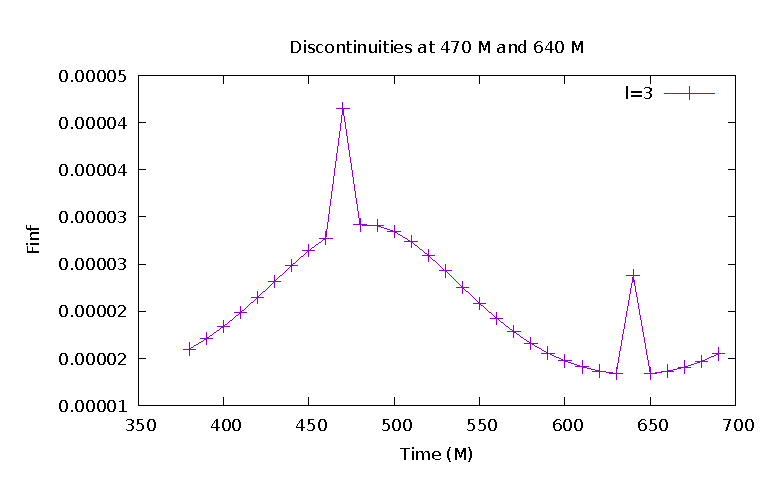
\includegraphics{finfovertimel3discontinuities}
\end{figure}

\begin{figure}
  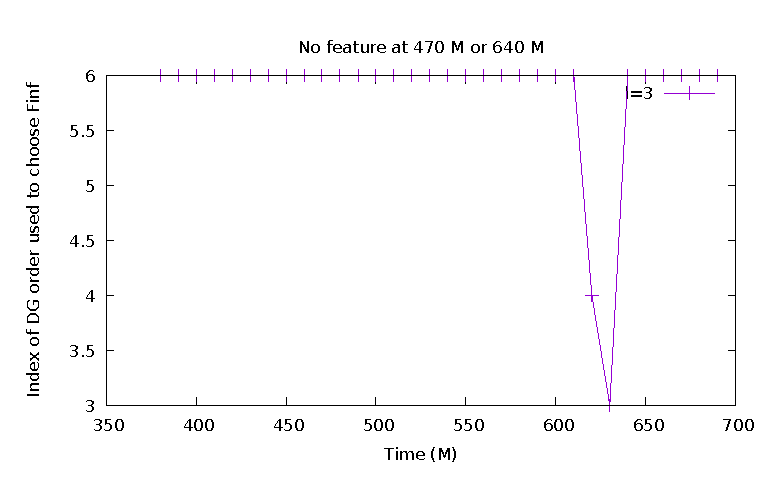
\includegraphics{nmaxovertimel3nofeaturesatdiscontinuitiesinfinf}
\end{figure}

\begin{figure}
  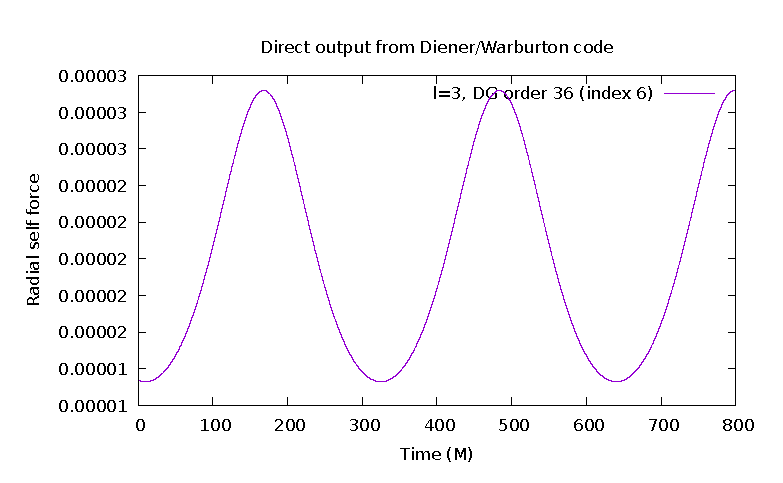
\includegraphics{psirl_l3_order36}
  \caption{470 M near perihelion, 640 M at aphelion}
\end{figure}

\begin{figure}
  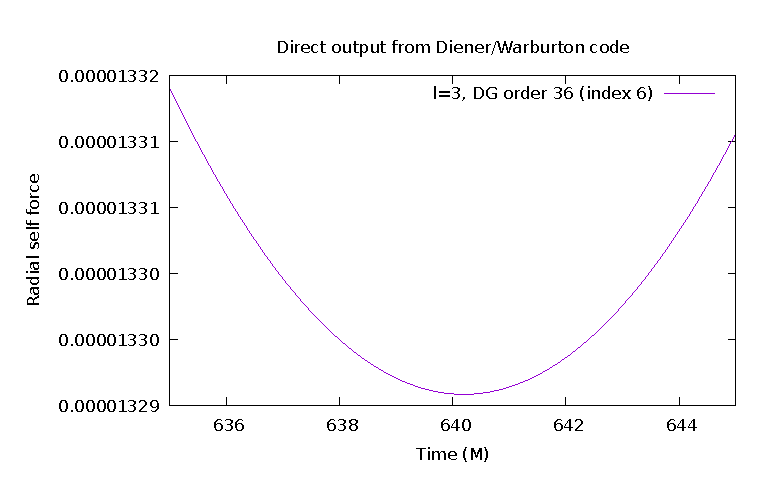
\includegraphics{psirl_l3_order36_t640zoom}
  \caption{No obvious features at aphelion}
\end{figure}

\end{document}
